\chapter[Password Selection and the Decoy Effect]{Password Selection and the Decoy Effect}\label{chap:decoy}

% Motivation
% users use weak passwords a
% users think l33t speak is more secure than other strategies (pasdjo finding)
% but this is not necessarily the case, passphrases might be a better alternative
% hard challenge: mental model of passphrases indicates users think they are too weak. 
% RQ: how can this be changed?
% RQ: reverse misconceptions with ``marketing'' \cite{Ashenden2013SecurityLikeSoap}
% RQ: in which way do suggestions influence self-selected passwords?



%TODO Result summary. 
\section{Background and Context}

Goal: influence / correct mental models of password strength, persuade users to consider alternative strategies. 

Criticism: this is unrealistic because memory interference effects prevent that this works for more than one account. -- yes, but for important accounts, this might still be worthwhile and people can more easily write down three words instead of an 8 character random sequence that might include ambiguous characters (0 and O); Kuo et al also say that writing down is a perfectly valid strategy \cite{Kuo2006HumanSelectionMnemonic}. (\todo{look up more researchers who argue in favor of writign down, e.g \cite{Kothari2017PasswordLogbooks} })

\subsection{Suggestions}
Main topic: suggesting methods, feedback, modifications
\cite{Ur2012HelpingUsersCreateBetterPasswords}
\cite{Shay2012CorrectHorseBatteryStaple}
\cite{Shay2014CanLongPasswordsBeSecureAndUsable}
\cite{Forget2008ImprovingPasswordsThroughPersuasion}


\subsection{The Decoy Effect}
The decoy effect was discovered through research in consumer psychology. Buying a product usually involves deciding between different alternatives. On a high level, products are easily comparable by their quality and price, so customers heavily rely on these two metrics. The two dimensions also build the foundation of the decoy effect. In one of the first experiments on ``asymmetric dominance'', Huber \etal illustrate decision-making processes with a simple example to decide between six-packs of beer that differ in price and quality \cite{Huber1982AsymetricallyDominated} (slightly adapted for simplicity): 
\begin{table}[!h]
\begin{tabular}{lrr}
	\textbf{Option} & \textbf{Price} & \textbf{Quality rating}\\
	(A) & \$4 & 50 \small{/100}\\
	(B) & \$6 & 70 \small{/100}\\
\end{tabular}
\end{table}

While option (A) is cheaper than (B), it is also lower in quality. Spending \$2 more, the buyer will get a higher-quality beer (B). With the information available at this point, it is hard to decide. 
Buyers may have a general preference for either lower price, or higher quality if all other factors are excluded. Imagine the vendor wants to sell more of beer (A) because margins are higher for that product. To achieve this, Huber \etal explored different ways of adding a third option:
\begin{table}[!h]
\begin{tabular}{lrr}
	\textbf{Option} & \textbf{Price} & \textbf{Quality rating}\\
	(A) & \$4 & 50 \small{/100} \\
	(B) & \$6 & 70 \small{/100}\\
	(C) & \$4 & 40 \small{/100} \\
\end{tabular} 
\end{table}

Product (C) is as expensive as (A), but falls behind in quality. Thus, buyers will make a ``better deal'' if they choose option (A) by comparison with (C). Options (B) and (C) are more difficult to compare, because both dimensions (price and quality) are higher in (B) and make it appear like an outlier. Option (C) is thus called the \textbf{decoy} that is \textit{dominated} by option (A) (\textbf{target}). Option (B) (the \textbf{competitor}) also beats the decoy, but the comparability between the target and the decoy boosts the favorability of the target. This is exactly what Huber \etal found, and which was later confirmed numerous times in different decision-making scenarios \cite{Ariely1995ExplanationSubjectiveDominance}. Adding the decoy has the potential to reverse existing preferences, making it a powerful tool for marketing and sales. The decoy itself often serves the sole purpose of making another item stand out, thus the underlying persuasion principles are \textbf{salience} and \textbf{framing}. Constructing the dimensions in a certain way is referred to as \textit{choice architecture} \cite{Thaler2010ChoiceArchitecture}, and is an important persuasive design strategy. 

Huber \etal stated that there is a specific combination of attributes to position the decoy (see Figure \ref{fig:decoy:general-construction}). Depending on the target, the decoy acts as range increasing (R, R*), frequency increasing (F), or both (RF). By extending the range on the dimension on which the \textit{competitor} is superior, the fixed difference between all items on that dimension is weighed less. Figure \ref{fig:decoy:beer-construction} illustrates this type of decoy placement for the sixpack example. The range of the quality is clearer after the decoy is added: before the span was [50;70], and afterwards [40;70]. The superiority of the competitor appears less significant, hence the higher price can seem unjustified. 

%- decoy: vendor does not intend to sell this, it acts as an unfavorable alternative that can be used as reference point / comparison.\\	

\begin{figure}[t]
	\begin{subfigure}[t]{0.49\textwidth}
		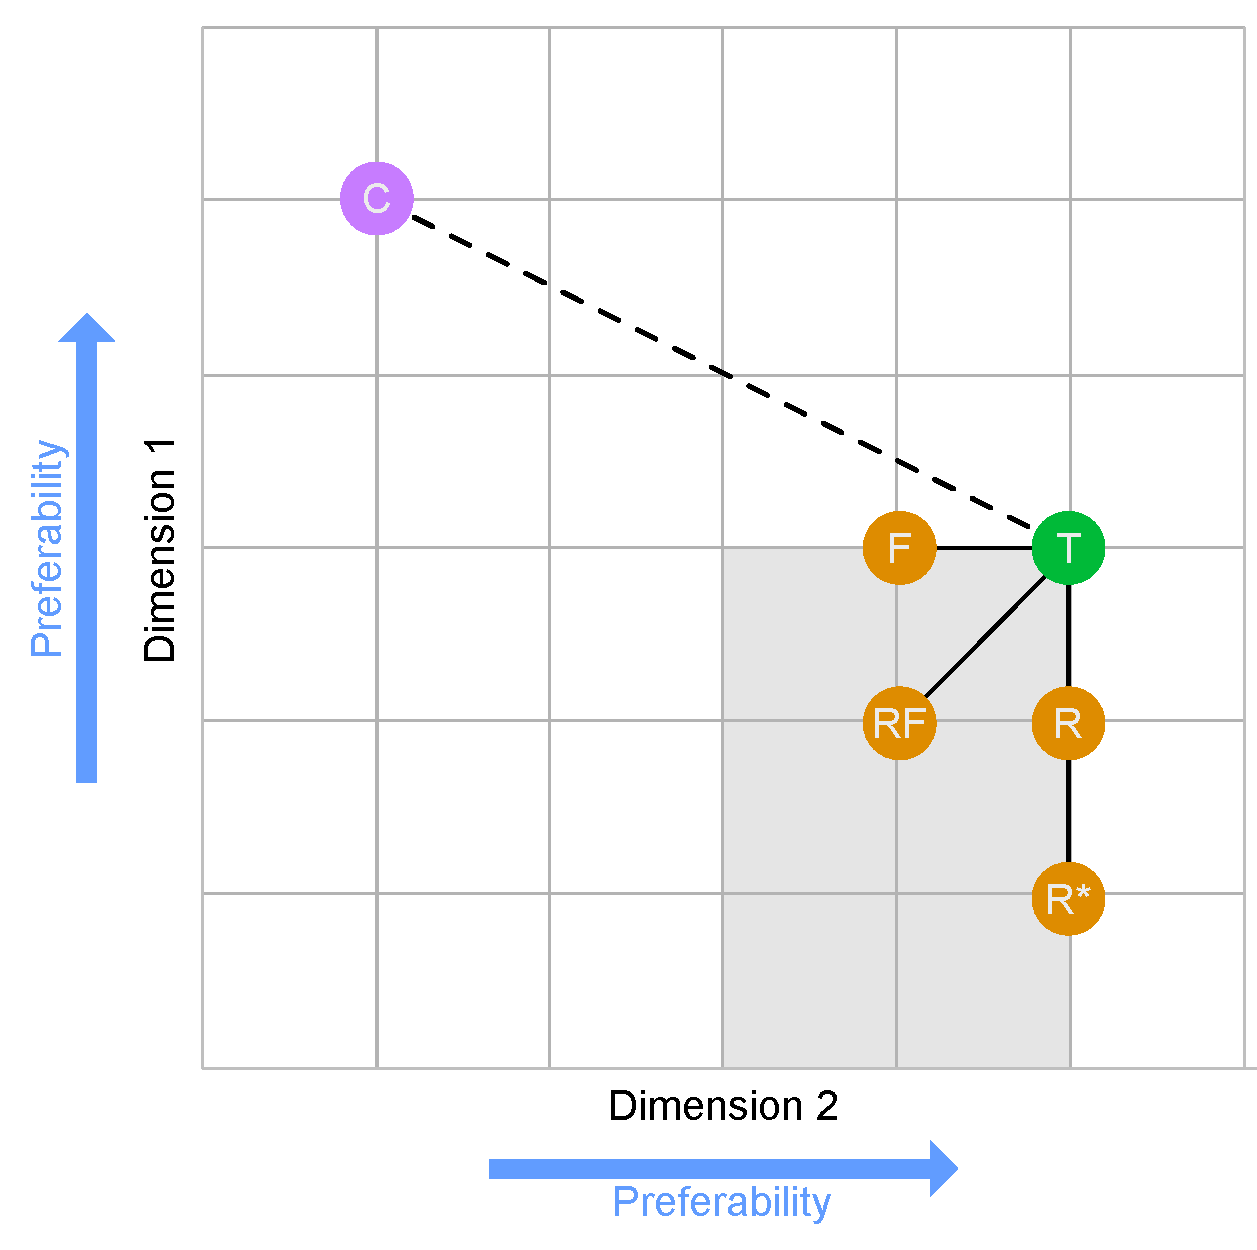
\includegraphics[width=\textwidth]{figures/decoy/decoy-dimensions-general}
		\caption{Decoy placement options \cite{Huber1982AsymetricallyDominated}}
		\label{fig:decoy:general-construction} 
	\end{subfigure}
	\begin{subfigure}[t]{0.49\textwidth}
		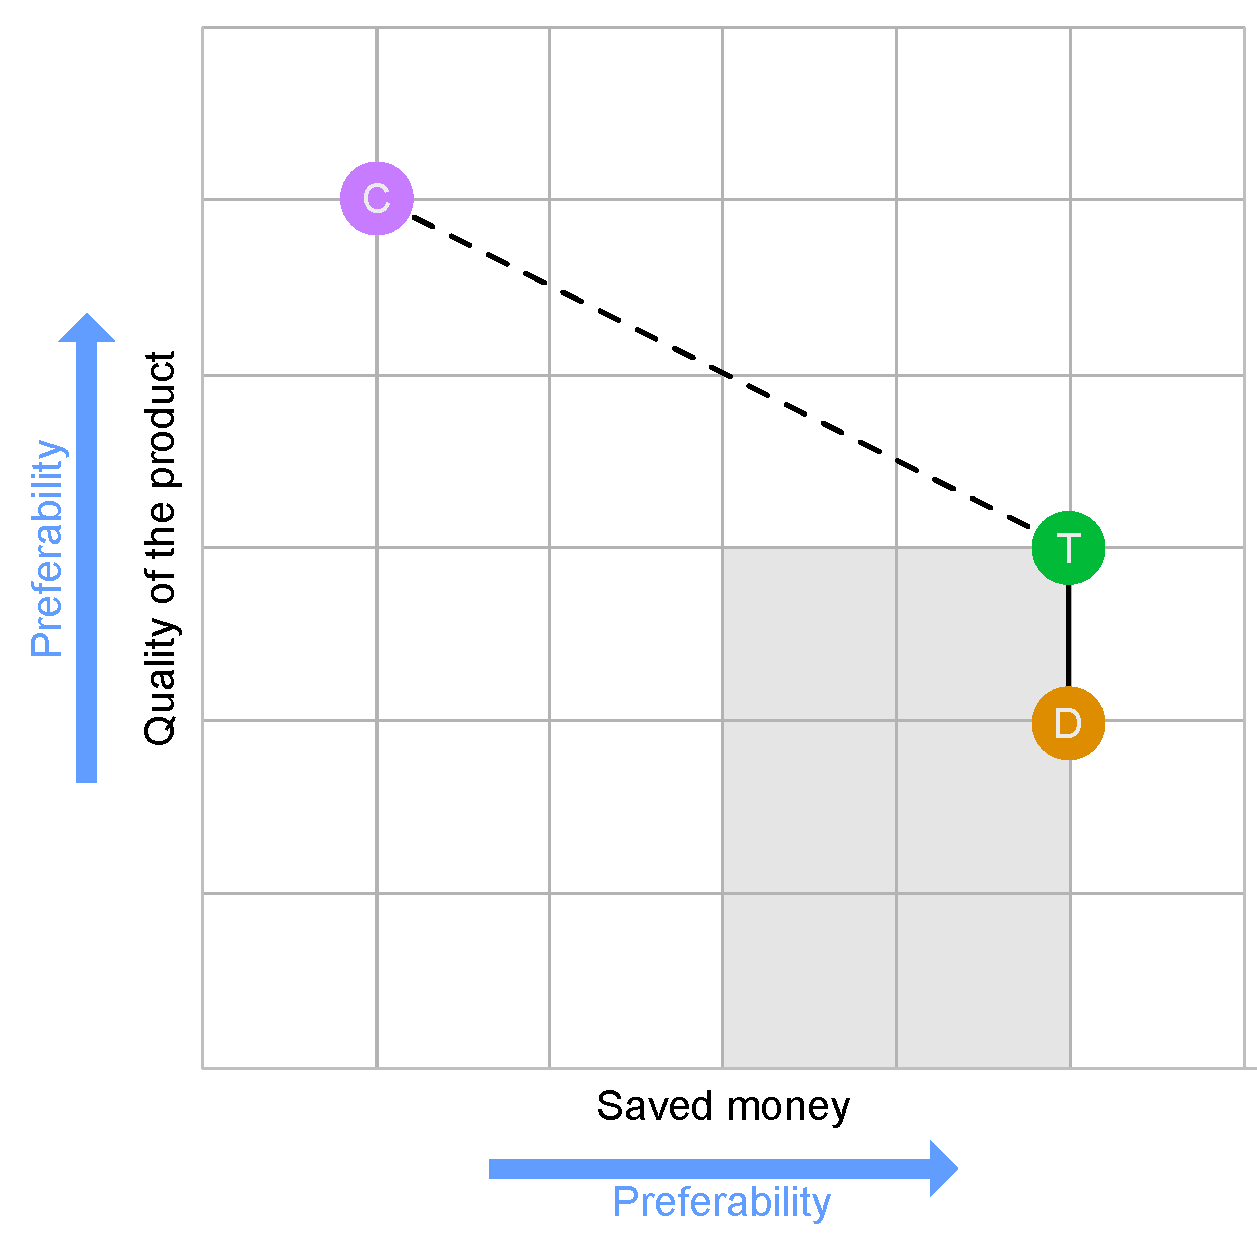
\includegraphics[width=\textwidth]{figures/decoy/decoy-dimensions-beer}
		\caption{Example choice architecture for sixpack of beers.}
		\label{fig:decoy:beer-construction} 
	\end{subfigure}
	\caption{
		General choice architecture overview to generate asymmetric dominance. 
		C = competitor, T = Target. The decoy can be placed at different positions in the spectrum, but needs to be dominated by the target (gray areay). Placement strategies for the decoy to increase the target's dominance: R = Range, R* = extreme range, F = frequency, RF = range and frequency.
	} 
\end{figure}

%- broader concept: framing, salience, anchoring. 
%- making choices, given a set of alternatives
%- using a decoy choice architecture to influence the preferred option 

\subsubsection{Example: Decoy Effects in the Real World}
Huber \etal's example has been adapted and used in the design of user interfaces. The vendor, i.e. a service provider, tries to steer users towards a particular direction that they see as favorable. For instance, location settings on an Android device show signs of a decoy pattern (see Figure \ref{fig:decoy:android-pattern}). From bottom to top, the ``device only'' mode activates the GPS module to determine the device's location. It is thus highly accurate outside of buildings, but does not work well inside. On the other hand, the ``battery saving mode'' works in both environments by using Google's online location services based on triangulation between network cells and surrounding WiFis. In urban areas and even inside buildings, it can achieve great accuracy, while it only roughly estimates locations in rural areas. The two accuracy-levels are thus comparable, but the ``battery saving mode'' does not require powering up additional antennae and modules, giving it a graspable advantage. The ``High accuracy'' mode combines both approaches and is thus the most battery consuming, but most versatile option. The ``battery saving'' can be seen as the target, because it provides the best trade-off in most situations. The ``device only'' mode is the decoy because it uses more battery, while the ``high accuracy'' mode is the competitor. Google requires the user to allow the collection of technical sensor data for the ``high accuracy'' and ``battery saving'' mode. Battery consumption is likely more important to users than location accuracy, which further suggests that the ``battery saving'' mode is indeed the targeted setting. 

\begin{figure}
	\begin{subfigure}[!t]{0.49\textwidth}
		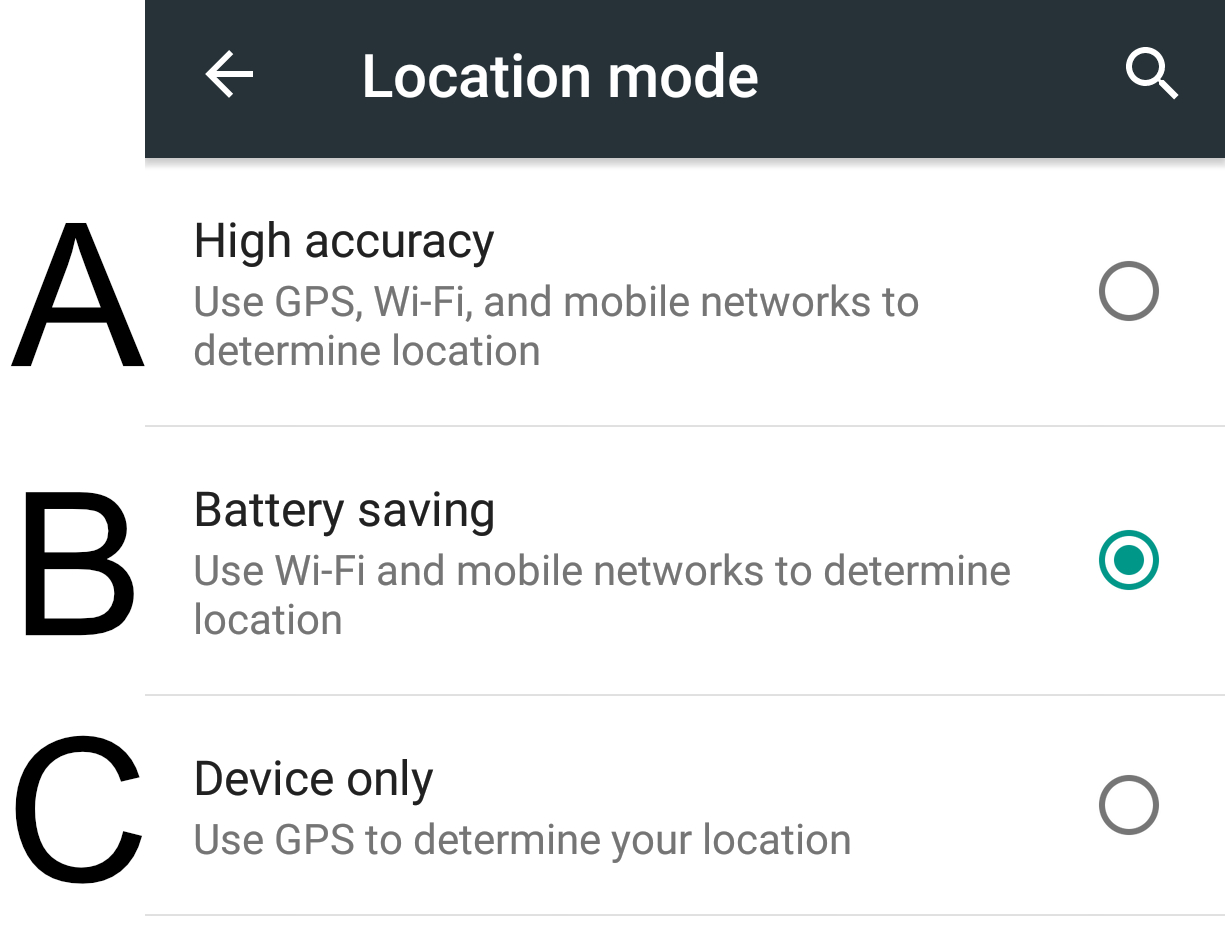
\includegraphics[width=\textwidth]{figures/decoy/Android_Location_Decoy}
	\end{subfigure}
	\begin{subfigure}[!t]{0.49\textwidth}
		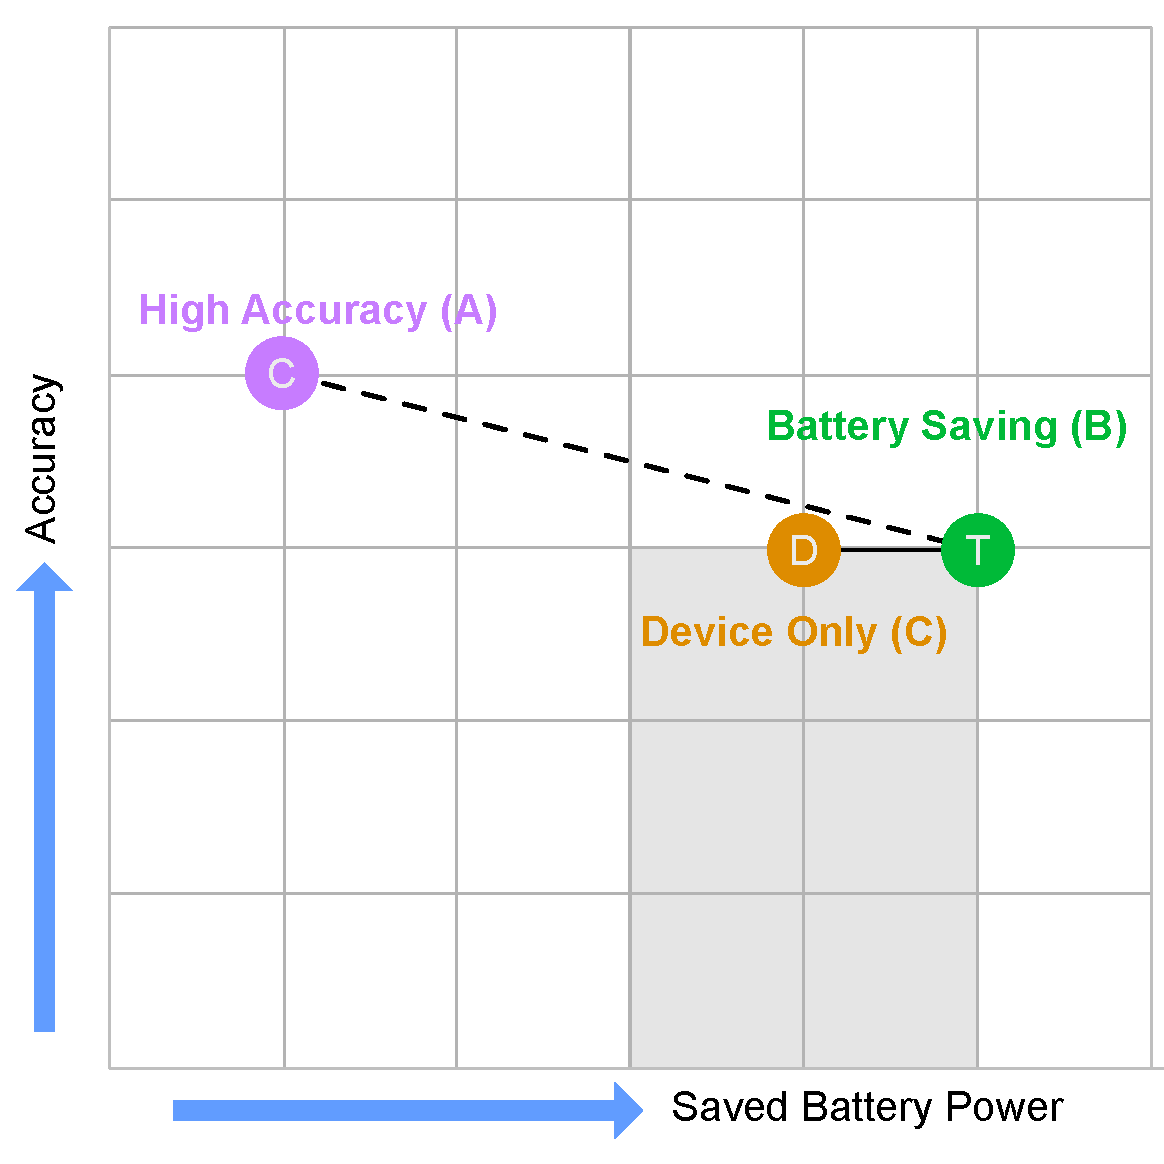
\includegraphics[width=\textwidth]{figures/decoy/decoy-dimensions-android}
	\end{subfigure}
	\caption{\label{fig:decoy:android-pattern}Location settings in Android show signs of a decoy pattern. The ``battery saving'' mode is targeted, because it does not activate the GPS module and can achieve comparable accuracy. Google benefits from collecting information on WiFi hotspots and network cells to improve their location service.} 
\end{figure}


\subsection{Choice Architecture in Security and Privacy}
The \gls{USEC} community has started to investigate the feasibility of behavioral economics principles in the design of security and privacy mitigations. Egelman \etal showed that choice architecture is highly relevant for privacy settings on mobile devices \cite{Egelman2013ChoiceArchitecture}. They explored how users value privacy-respecting apps and how they make decisions from a list of applications. To measure preferences, they put monetary values and discounts on permissions like accessing the Internet or using device location. Participants in their study showed clear decision-making patterns that were influenced by the price and type of permission. Therefore, Egelman \etal concluded that a certain choice architecture can guide users towards a more ``rational behavior''. 

Knijnenburg \etal \cite{Knijnenburg2013MorePrivacyOptions} explored the \textit{choice proliferation} phenomenon in location-privacy settings. The principle indicates that people become choice averse with an increasing number of options. In their study, they observed that participants were strongly influenced by the number of available options to share their location. Without specifically mentioning it, they also used a \textit{decoy} option that was extremely unfavorable, but triggered a change in preference. In another study, Korff and Böhme showed that the granularity of privacy settings on a business social network can have similar effects: participants in their study tended to stick with default settings and were also less satisfied with their choices \cite{Korff2014TooMuchChoice}. Acquisiti \etal showed that such architectures can nudge users towards certain settings \cite{Acquisti2017NudgesPrivacySecurity}. 

Regarding passwords, only few publications mention the use of choice architectures. Renaud \etal evaluated a wide range of nudges to make users of a university platform pick a stronger passwords. They concluded that the tested architectures were fairly ineffective in achieving this goal, but there might have been other more effective solutions beyond their designs. Before our own investigation, no study that we are aware of has explored the decoy paradigm for passwords. 

% might be mentioned briefly:%
%\cite{Wang2014PrivacyNudgesFacebook}
%\cite{Malkin2017PersoanlizedSecurityMessaging}
%\cite{Jameson2011PreferentialChoice}

\section{Designing Password Choice Architecture}
% Briefly point to first exploration report to mention a design that failed. 
We aimed to craft a nudge that persuades users to create stronger passwords. Respecting the principle of the opportune moment, we opted for account creation contexts. To emulate a situation that is comparable to buying one out of several product alternatives, we show suggestions beneath the password field where the user enters their choice (see Figure \ref{fig:decoy:design-architecture-prolific}). We ended up with this design after identifying opportunities of strength feedback on the user's password and on the suggestions (i.e. feed-forward). To that end, we had created several prototypical choice architectures and rapidly evaluated them in the lab and online (see technical report \cite{Seitz2016DecoyEffectReport}). The final architecture implements the propositions in Huber \etal's framework (see Figure \ref{fig:decoy:dimensions-prolific}).

\begin{figure}[t]
	\begin{subfigure}[!t]{0.49\textwidth}
		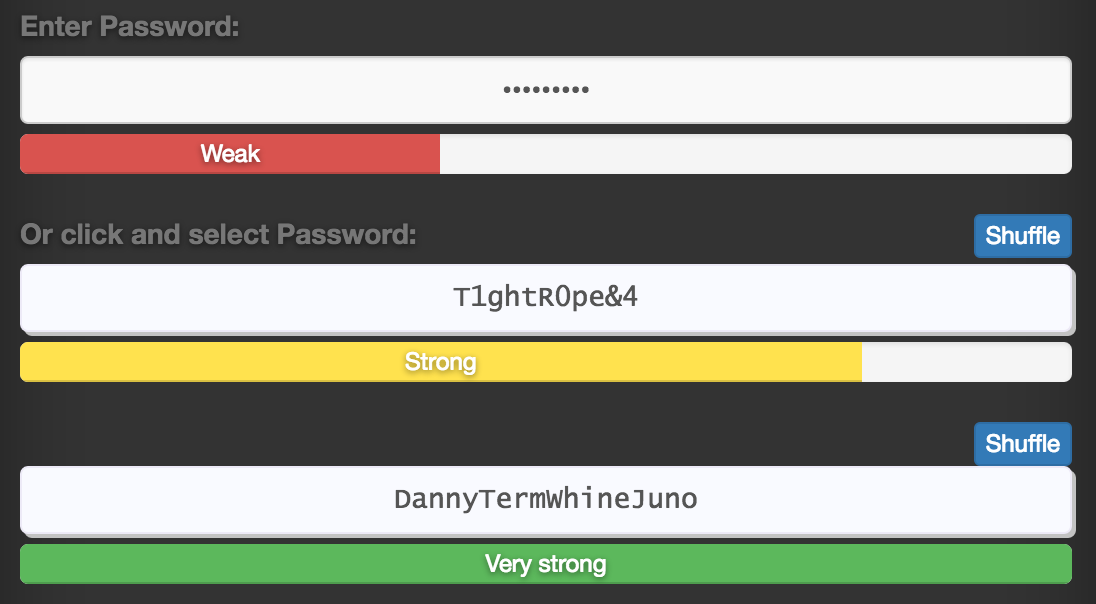
\includegraphics[width=\textwidth]{figures/decoy/generator_prolific_3}\label{fig:decoy:screenshot-prolific}
	\end{subfigure}
	\begin{subfigure}[!t]{0.49\textwidth}
		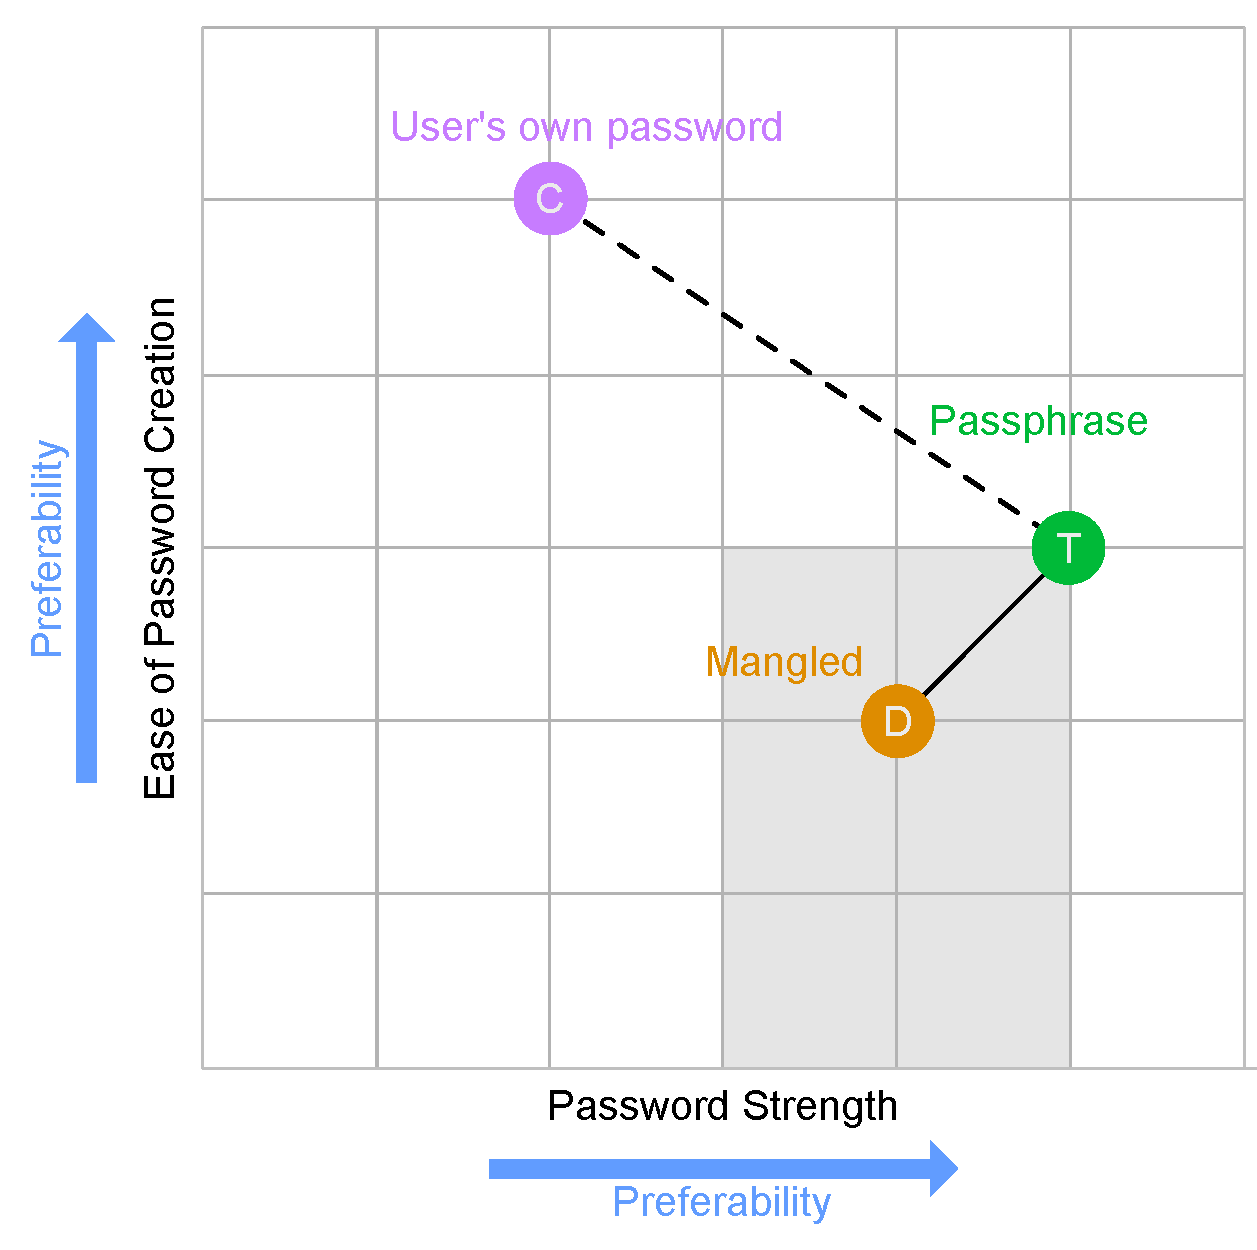
\includegraphics[width=\textwidth]{figures/decoy/decoy-dimensions-prolific}\label{fig:decoy:dimensions-prolific}
	\end{subfigure}
	\caption{\label{fig:decoy:design-architecture-prolific}Choice architecture and decoy placement as evaluated in the online experiment. } 
\end{figure}

The key to password choice architecture is the user's own password. It has to be seen as the \textbf{competitor}. Service providers will want accept the user's own password, because they want make sure users sign up. On the other hand, they want to avoid attacks on user accounts, which is why they likely encourage using a stronger password. This is the \textbf{target}. In our design, we opted for a \textit{passphrase} as target for several reasons: only few users create secure passphrases as their primary credentials \cite{Ur2015PWCreationLab}; passphrases provide usability and memorability benefits \cite{Keith2009PassphraseDesign}; self-selected passphrases often do not provide the desired security benefits \cite{Bonneau2012LinguisticProperties}, which can be mitigated by supplying users with a combination of random words \cite{Shay2012CorrectHorseBatteryStaple}. 

To make the passphrase preferable over the competitor, a decoy needs to be carefully positioned along the two dimensions such that it is closer to the target than to the competitor. Moreover, it needs to be dominated at least in one dimension by the target. To achieve this, we identified ``ease of use'' and ``security benefits'' as two feasible dimensions of the choice architecture. We opted for a range-frequency decoy (see Figure \ref{fig:decoy:general-construction}) where the target dominates the decoy in \textit{both} dimensions, because effects are more likely to be detected this way. A typical-length \textit{mangled} password fulfills the criteria. The richer character set includes symbols that require the Shift/Alt keys to enter them. Thus, the ease of creation is lower than that of a passphrase (dimension 1). At the same time, typical mangling strategies only slightly contribute to password strength, which we confirmed in Chapter \cite{chap:pasdjo}. Passphrases are considered stronger by several estimators. Consequently, mangled passwords are dominated by passphrases regarding strength (dimension 2). Figure \ref{fig:decoy:dimensions-prolific} illustrates the positioning along the two dimensions.

\section{Quantitative Evaluation}
We ran an online experiment to evaluate the efficacy of our decoy choice architecture for passwords. We formed the following hypotheses about the outcome:
\begin{description}
	\item[H0] Participants' self-selected passwords are comparable in strength and memorability, regardless of the presence of a password suggestion (Nullhypothesis). 
	\item[H1] The presence of a single password suggestion will lead to slightly stronger passwords.
	\item[H2] The presence of two suggested passwords that follow a decoy choice architecture regarding strength and ease of use will lead to stronger passwords that resemble the target suggestion. 
\end{description}

\subsection{Method}
% study design, independent variable
The study implemented a between groups design. The main task was creating a new password under one of four treatments. ``Suggestion architecture'' served as independent variable with three levels: \textbf{Passphrase}, \textbf{Mangled}, and \textbf{Decoy}. Each level was tested with a separate participant group. In the Passphrase condition, participants were suggested a single passphrase consisting of four words. Analogously, a higher-complexity password is displayed in the Mangled condition. The Decoy group received both the target passphrase and the complex decoy password as alternative suggestions to their own password. Having study conditions with single suggestions allowed us to measure the impact of the decoy effect. All suggestions are accompanied by visual and textual representations of zxcvbn scores. The labels for the different strength scores were \textit{very weak, weak, ok, strong, very strong}. To obtain a baseline for comparison, there were no password suggestions for the \textbf{Control} group. However, participants in this group received strength feedback allowing us investigate the impact of suggestions. 

%dependent variables
We did not collect plain text passwords to ethically deal with participants disclosing their real passwords. Instead, we used modified the zxcvbn library by stripping all sensitive information\footurl{https://gist.github.com/TobiasSeitz/e27a867535b82f6cf9a6ae6140da8b81}{06.03.2018}, and analyzed participants' passwords on the fly. These \textit{meta statistics} served as dependent variables and were saved to a regular database. Most notably, they describe the password topology (length, number of upper-/lowercase, digits, symbols, and chunks), estimated guess numbers and the zxcvbn score. Scores range from 0 (weak) to 4 (strong), while guess number estimates are open-end. Another dependent variable was memorability which was measured by a successful authentication three days after password selection. To achieve this, we hashed passwords with a secure one-way function (PHP's \texttt{password\_hash()}) and compared hashes afterwards. If they matched, the password was correct, thus this is a binary metric.

\subsubsection{Prototype}
For the purpose of the study, we implemented the concept as web-prototype based on HTML and JavaScript. As foundation for the generating passwords in all conditions, we relied on the Diceware dictionary\footurl{http://world.std.com/\~reinhold/diceware.wordlist.asc}{06.03.2018} consisting of 5823 words. It provides a good spectrum of common and uncommon words of varying length. To generate the passphrase (target), four words were randomly combined and capitalized individual words. As shown in Chapter \ref{chap:pasdjo} zxcbvn rates four-word passwords with its highest score. The randomness of generated passwords allows us to calculate their entropy. Each word has an estimated entropy of $(log_2(5823) \approx 12$ bits. Combining four words randomly thus results in a total entropy of approximately $ (2^{12})^4 = 48$ bits for passphrases.

For the decoy and the mangled password condition, the prototype modifies a randomly selected word from a smaller subset of the Diceware list. The subset only includes words longer than eight characters, giving a total of 687 candidates. The first letter of the word, and a second randomly chosen character are capitalized. Two letters are substituted by similarly-looking digits to inspire a \textit{l33t} character. For instance, the letter ``o'' was replaced with the digit ``0''. Finally, a random symbol and digit are appended to the word. The resulting decoy password consists of four different character classes (LUDS). 

We anticipated that the generated passwords are exceptionally unattractive in some cases, e.g. if passphrases consist include uncommon, hardly memorable words, e.g. \texttt{GirthInflixThineAegis}. To make them more appealing, the prototype provides a \textit{shuffle} button that gives a new combination of words (see Figure \ref{fig:decoy:screenshot-prolific}). The mangled password can also be re-generated. Another feature to lower barriers to take one of the suggested passwords was the opportunity to transfer it to the password field with a single click. However, to facilitate memorization, participants needed to manually type the password into the confirmation field. 

\subsubsection{Procedure}
The experiment consisted of two parts that were carried out on separate days. The initial step included the password selection task and usability assessment among other qualitative metrics. Participants were invited to return for the second part of the study three days later. This follow-up step included memorability assessment and further qualitative feedback to help us understand the data.

The first part started with a thorough briefing about the collected data and asked for consent. The same web-page introduced the scenario for the task: Participants were asked to imagine creating a new password for their already existing email account. The page displayed the password fields and suggestions. Participants were randomly assigned to one of the four treatment groups, so the type and number of suggestions depended on this assignment. Once the password was successfully confirmed, participants were asked to fill out a brief questionnaire mostly consisting of 5-point scale items on attitudes and password behaviors. At the end of the first part, the web-page displayed a confirmation code that participants had to copy over to the prolific platform to mark the survey as done. 

Three days afterwards, we invited the participants to return and complete the second part. They were asked to provide the password they had remembered, but we did not validate 

\subsubsection{Recruitment and Sample}
Following best practices in password research, we leveraged crowd-sourcing tools to elicit the data. Recruitment took place through the research platform Prolific\footurl{https://prolific.ac}{06.03.2018}, which is comparable to Amazon's Mechanical Turk solution. Participants were screened for age (older than 18 years), and they had to be located in either the UK or in USA. The region restriction was introduced because Prolific has a larger user base in those countries. To ensure quality of the data, we required a past survey completion rate of at least 95\%. This is a common metric for the reliability of a crowd-worker \cite{Ross2010WhoAreTurkers}. 

From the 106 respondents who started the experiment, we had to reject seven because the study completion code was wrong or missing, or because the questionnaire was insufficiently filled out or completion times were outliers ($> 3*SD$). The remaining 99 participants received invitations to return, which 97 people did. There were another fourteen incomplete responses or wrong study codes. Hence, the resulting N of our data set is $N = 84$ valid, complete responses in both parts. Group sizes were $n=18$ in Control, $n=24$ in Passphrase, $n=21$ in Mangled, and $n=20$ in Decoy. On average, participants were 30 years old ($SD=10$). 42\% were female. The majority (78\%) was employed, 12\% were students, 10\% were unemployed. Participants reportedly possessed nine online accounts that they regularly use ($SD=5.6$). 

%no CS students: just like in \cite{Wash2016UnderstandingPasswordChoices}

%live deployment. 
%users could shuffle. 

\subsection{Survey Results}
Mostly focus on the contents of the paper here
-- General strategy (create logistic regression).


%\subsection{Live-Deployment Data}
%Talk about a couple of findings of the Roskilde dataset. 
% nah. there's no time for that now. 
%TODO add screenshot from roskilde sign-up. 

\subsection{Limitations}
No data on memorability
zxcvbn as strength metric.

\section{Discussion}

\subsection{The Ineffectiveness of the Decoy Effect}
- users were still unaware of the two dimensions: usability and security. the ease of use was still too low to compete against their own passwords. 
- the original experiments were within subjects. counterbalanced order. start out with three options --> two in the second part and vice versa. maybe this could have helped bring forward the desired nudging effect. 

\subsection{Creativity Support}
As we have seen in chapter \ref{chap:pasdjo}, users know fairly well what makes a strong password. Thus, we can explain the stronger influence of the passphrase in several ways. There might be a gap between password strength perception and selection that is due to \textit{creativity}. It might be easier for people to decide upon a stronger password if they actually see it. This, however, will not work, if the password is absolutely unrelated to the person because this increases memorization efforts. 

Creativity is usually associated with the ``Openness'' personality trait (see chapter \ref{chap:pws_and_personality}). So we can suspect that people who show less of this trait might be more susceptible to a password suggestion. 

mental model influenced? -- look at qualitative data. 


\begin{figure}
	\centering
	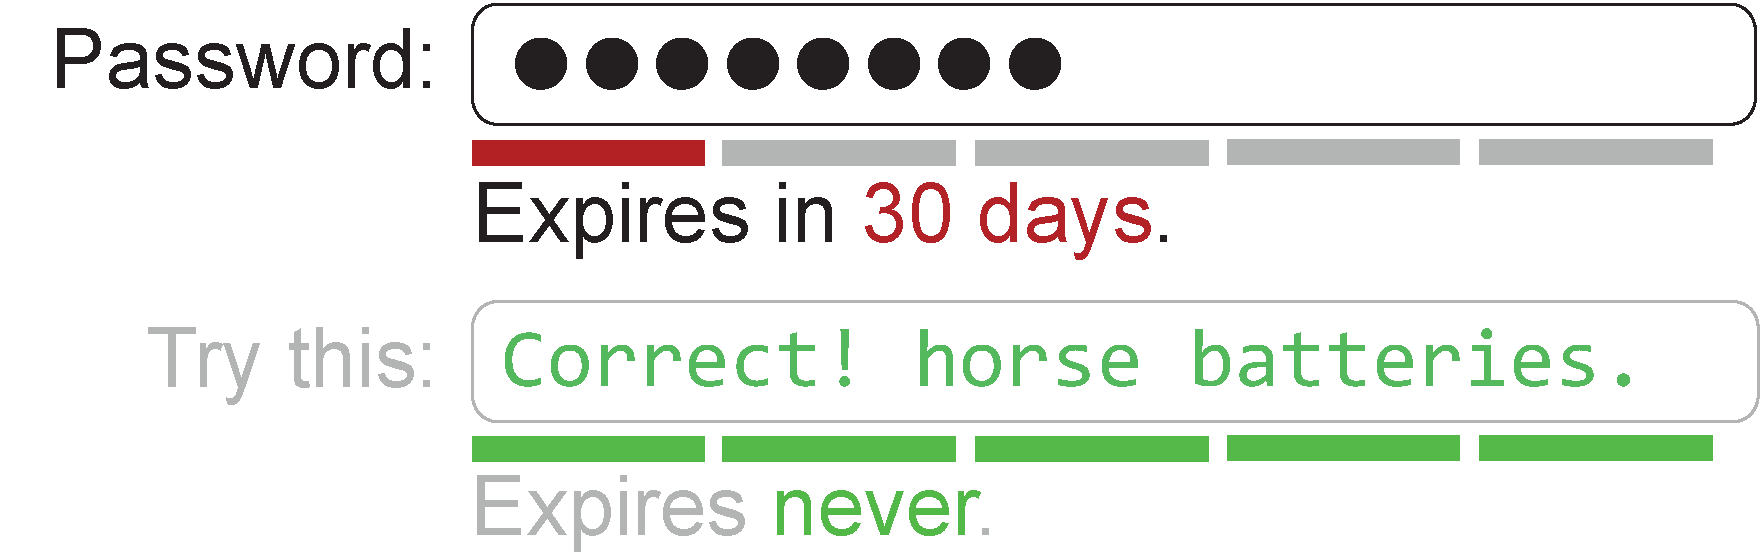
\includegraphics[width=0.7\linewidth]{figures/decoy/expire_mockup}
	\caption{\label{fig:decoy:expiremockup}Suggestion accompanied by enforced password expiration information.}
\end{figure}


\subsection{Application Areas}
it is not feasible to make users pick strong passwords for all accounts.
they already keep a list of ``important'' accounts that they wish to protect well, but stay in charge, so picking a strong memorable password for this type of account is vital to them. 

also, master passwords as gate-keeper to a larger number of passwords. 

\subsection{Personas}
which personas might be most most receptive to suggestions?

\section{Conclusion}

The idea we put forward in \cite{Seitz2016DecoyEffect} (see Figure \ref{fig:decoy:expiremockup}) was very recently evaluated by Renaud and Zimmermann \cite{Renaud2018NudgingFolks}. They concluded that providing a graspable benefit is the key to effectively nudge users towards stronger passwords. 

\section{Take-Aways}



